\documentclass[Nike]{tuberlinbeamer}

\usepackage[ngerman]{babel}  % 'babel' muss geladen werden
\usepackage[utf8]{inputenc}  % optional, aber empfehlenswert
\usepackage[T1]{fontenc}

\usepackage{svg}
\usepackage[export]{adjustbox}
\usepackage{amssymb}

% Die ueblichen Angaben
\title{PAVOOC - Prediction and visualization of on- and off-targets for CRISPR}
\subtitle{Master thesis}
\author[Moritz Schäfer]{Moritz Schäfer}
\institute{Technische Universität Berlin \& Bayer Pharma}

% Eigenes Logo einfuegen:
\renewcommand{\pathtomylogo}{meinlogo}

\begin{document}

\begin{frame}
\maketitle
\end{frame}


% \begin{frame}
% \frametitle{Outline}
% \tableofcontents
% \end{frame}

\section{Background}
\begin{frame}{Background}
  \begin{figure}
    \hspace*{0.2in}
    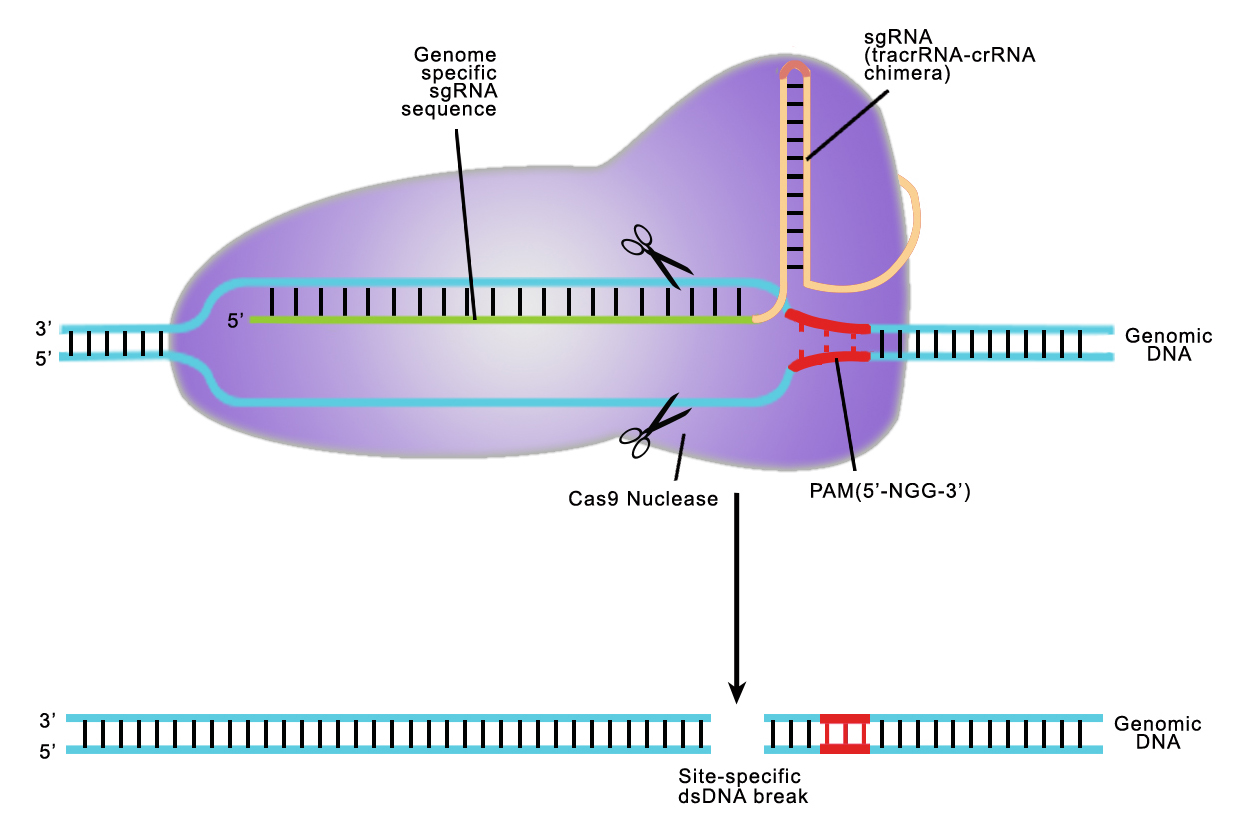
\includegraphics[width=0.57\linewidth,left]{Doudna-art-crop.jpg}
  \end{figure}
  \begin{itemize}
    \item Knockout experiments used in drug target validation
    \item Sequence (partially) determines efficacy
  \end{itemize}
\end{frame}

\section{Problem}

\begin{frame}
  \frametitle{Problem}
  \begin{itemize}
    % \item Many tedious and incomplete guide design tools \\
    %   \texttt{./guidesearch | ./convert\_output.sh | ./score\_guides > output.csv}
    \item Guide prediction scores still vary in performance
    \pause
    \item A lot of manual labor for guide selection \\
      \includegraphics[width=0.7\linewidth,left]{xlswork.png}
    \pause
    \item Non-frame-shift indels cannot be circumvented
      \includegraphics[width=0.6\linewidth,left]{nonframeshift.png}
    \pause
    \item Cancer cellline data affects certain guides
      \includegraphics[width=0.3\linewidth,left]{guide_snp.png}
  \end{itemize}
\end{frame}

\section{Solution}

\begin{frame}{Solution}
  \begin{itemize}
    \item Cutting-edge guide efficacy scoring
    \item All-in-one guide design tool
    \item Web-based
      % So it is easy to use for pure biologists only
    \item Functional domain-aware
    \item Incorporate cancer cellline data
  \end{itemize}
\end{frame}

% lets go into detail of the most important problem I target in my project.

\subsection{Guide efficacy prediction}

\begin{frame}{Guide efficacy prediction -- Dataset}
\begin{table}[]
    \centering
    \begin{tabular}{cc}
        \textbf{Guide} & \textbf{Measured efficacy} \\ \hline
\texttt{GTAGGGGTCCGTACTCAGCAAGG} & 0.86 \\
\texttt{ACACTGCCGAGCGATGAGGATGG} & 0.42 \\
\texttt{AAGGTGAAGGAGGATGCGGCGGG} & 0.53 \\
\texttt{GAAAAGATAGGTCACTGACCCGG} & 0.12 \\
\texttt{GCAAGTCACTGAGTGCAGAACGG} & 0.73 \\
\texttt{GCATTGGTAAGCGCACAGGAAGG} & 0.70 \\
\texttt{AAGACTGGCGCATGGTCCACTGG} & 0.57 \\
\texttt{...} & ... \\
    \end{tabular}
\end{table}
\begin{itemize}
  \item 5310 data rows
  \item Efficacy relates to cell proliferation after CRISPR application
\end{itemize}
\begin{flushright}
  \tiny
  ``Optimized sgRNA design to maximize activity and minimize off-target effects of CRISPR-Cas9'', 2016, John G. Doench et al.\
\end{flushright}
\end{frame}

\begin{frame}{Conservation features}
  \begin{figure}
    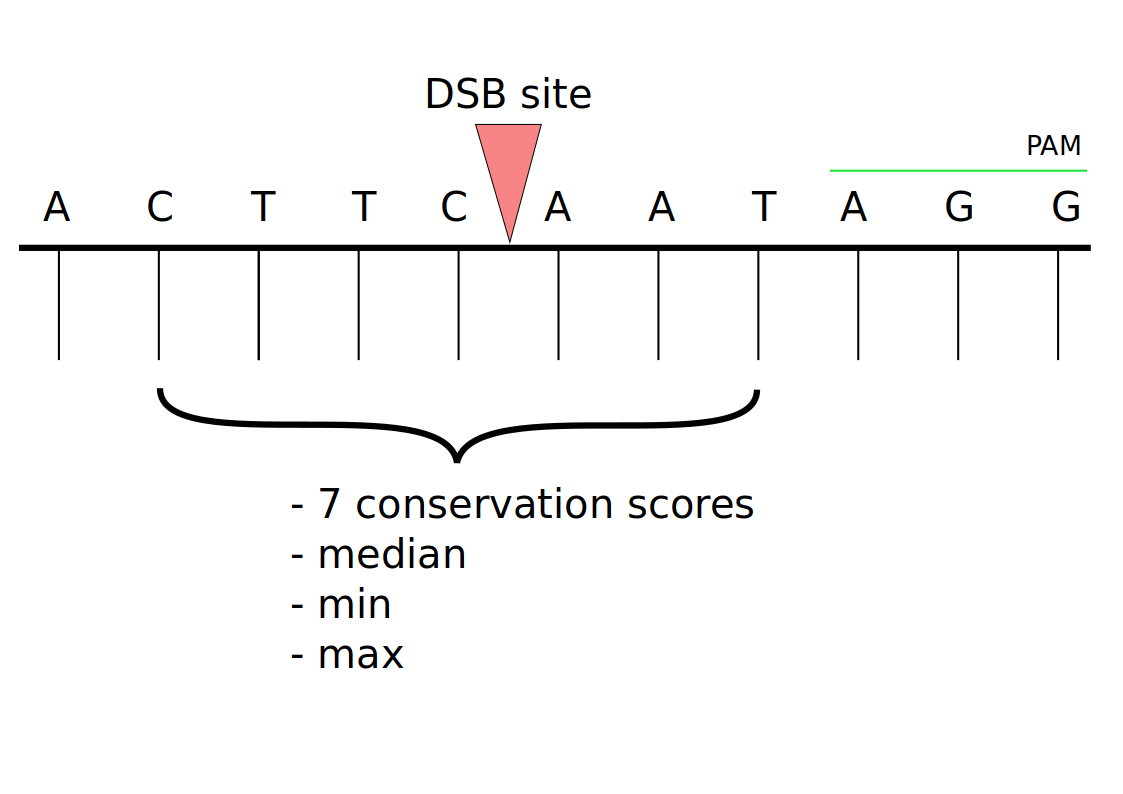
\includegraphics[width=0.45\linewidth]{Conservation_features.png}
    \hspace*{0.1in}
    \includegraphics[width=0.45\linewidth]{conservation_correlations.png}
  \end{figure}
  \hspace*{3.1in}
  $p_{max}=0.0043$

\end{frame}

\begin{frame}{Conservation feature results}
  Comparison of 100 runs on adaboost
  \begin{figure}
    \includegraphics[width=0.45\linewidth]{adaboost_conservation_comparison.png}
    \hspace*{0.1in}
    \includegraphics[width=0.45\linewidth]{adaboost_conservation_comparison_boxplot.png}
  \end{figure}
\end{frame}

\begin{frame}{Deep Learning architecture}
  \begin{flushright}
    \tiny
      ``Predicting the sequence specificities of DNA-and RNA-binding proteins by deep learning'', 2015, B. Alipanahi et al.\
  \end{flushright}
  \vspace*{-0.3in}
  \begin{figure}
    \includegraphics[width=0.65\linewidth]{CNN34_layout.png}
    \pause
    \includegraphics[width=0.25\linewidth]{fake_dnn_comparison.png}
  \end{figure}

  Conclusion: Deep Learning can improve guide efficacy prediction
\end{frame}

% To build the web application, I first developed a data processing pipeline that gathers various relevant data sources, preprocesses them and stores them in an easy to access format in a database. From this data I also generated the BED files being using in the Sequence Browser.
\begin{frame}{Architecture}
  \begin{figure}
    \centering
    \includegraphics[width=0.65\linewidth]{architecture.png}
  \end{figure}
\end{frame}

% So let me show you how guides are designed for an experiment with a given cellline and a set of targeted genes.

\subsection{Web Application}

\begin{frame}[fragile]{Application overview}
  \begin{figure}
    \centering
    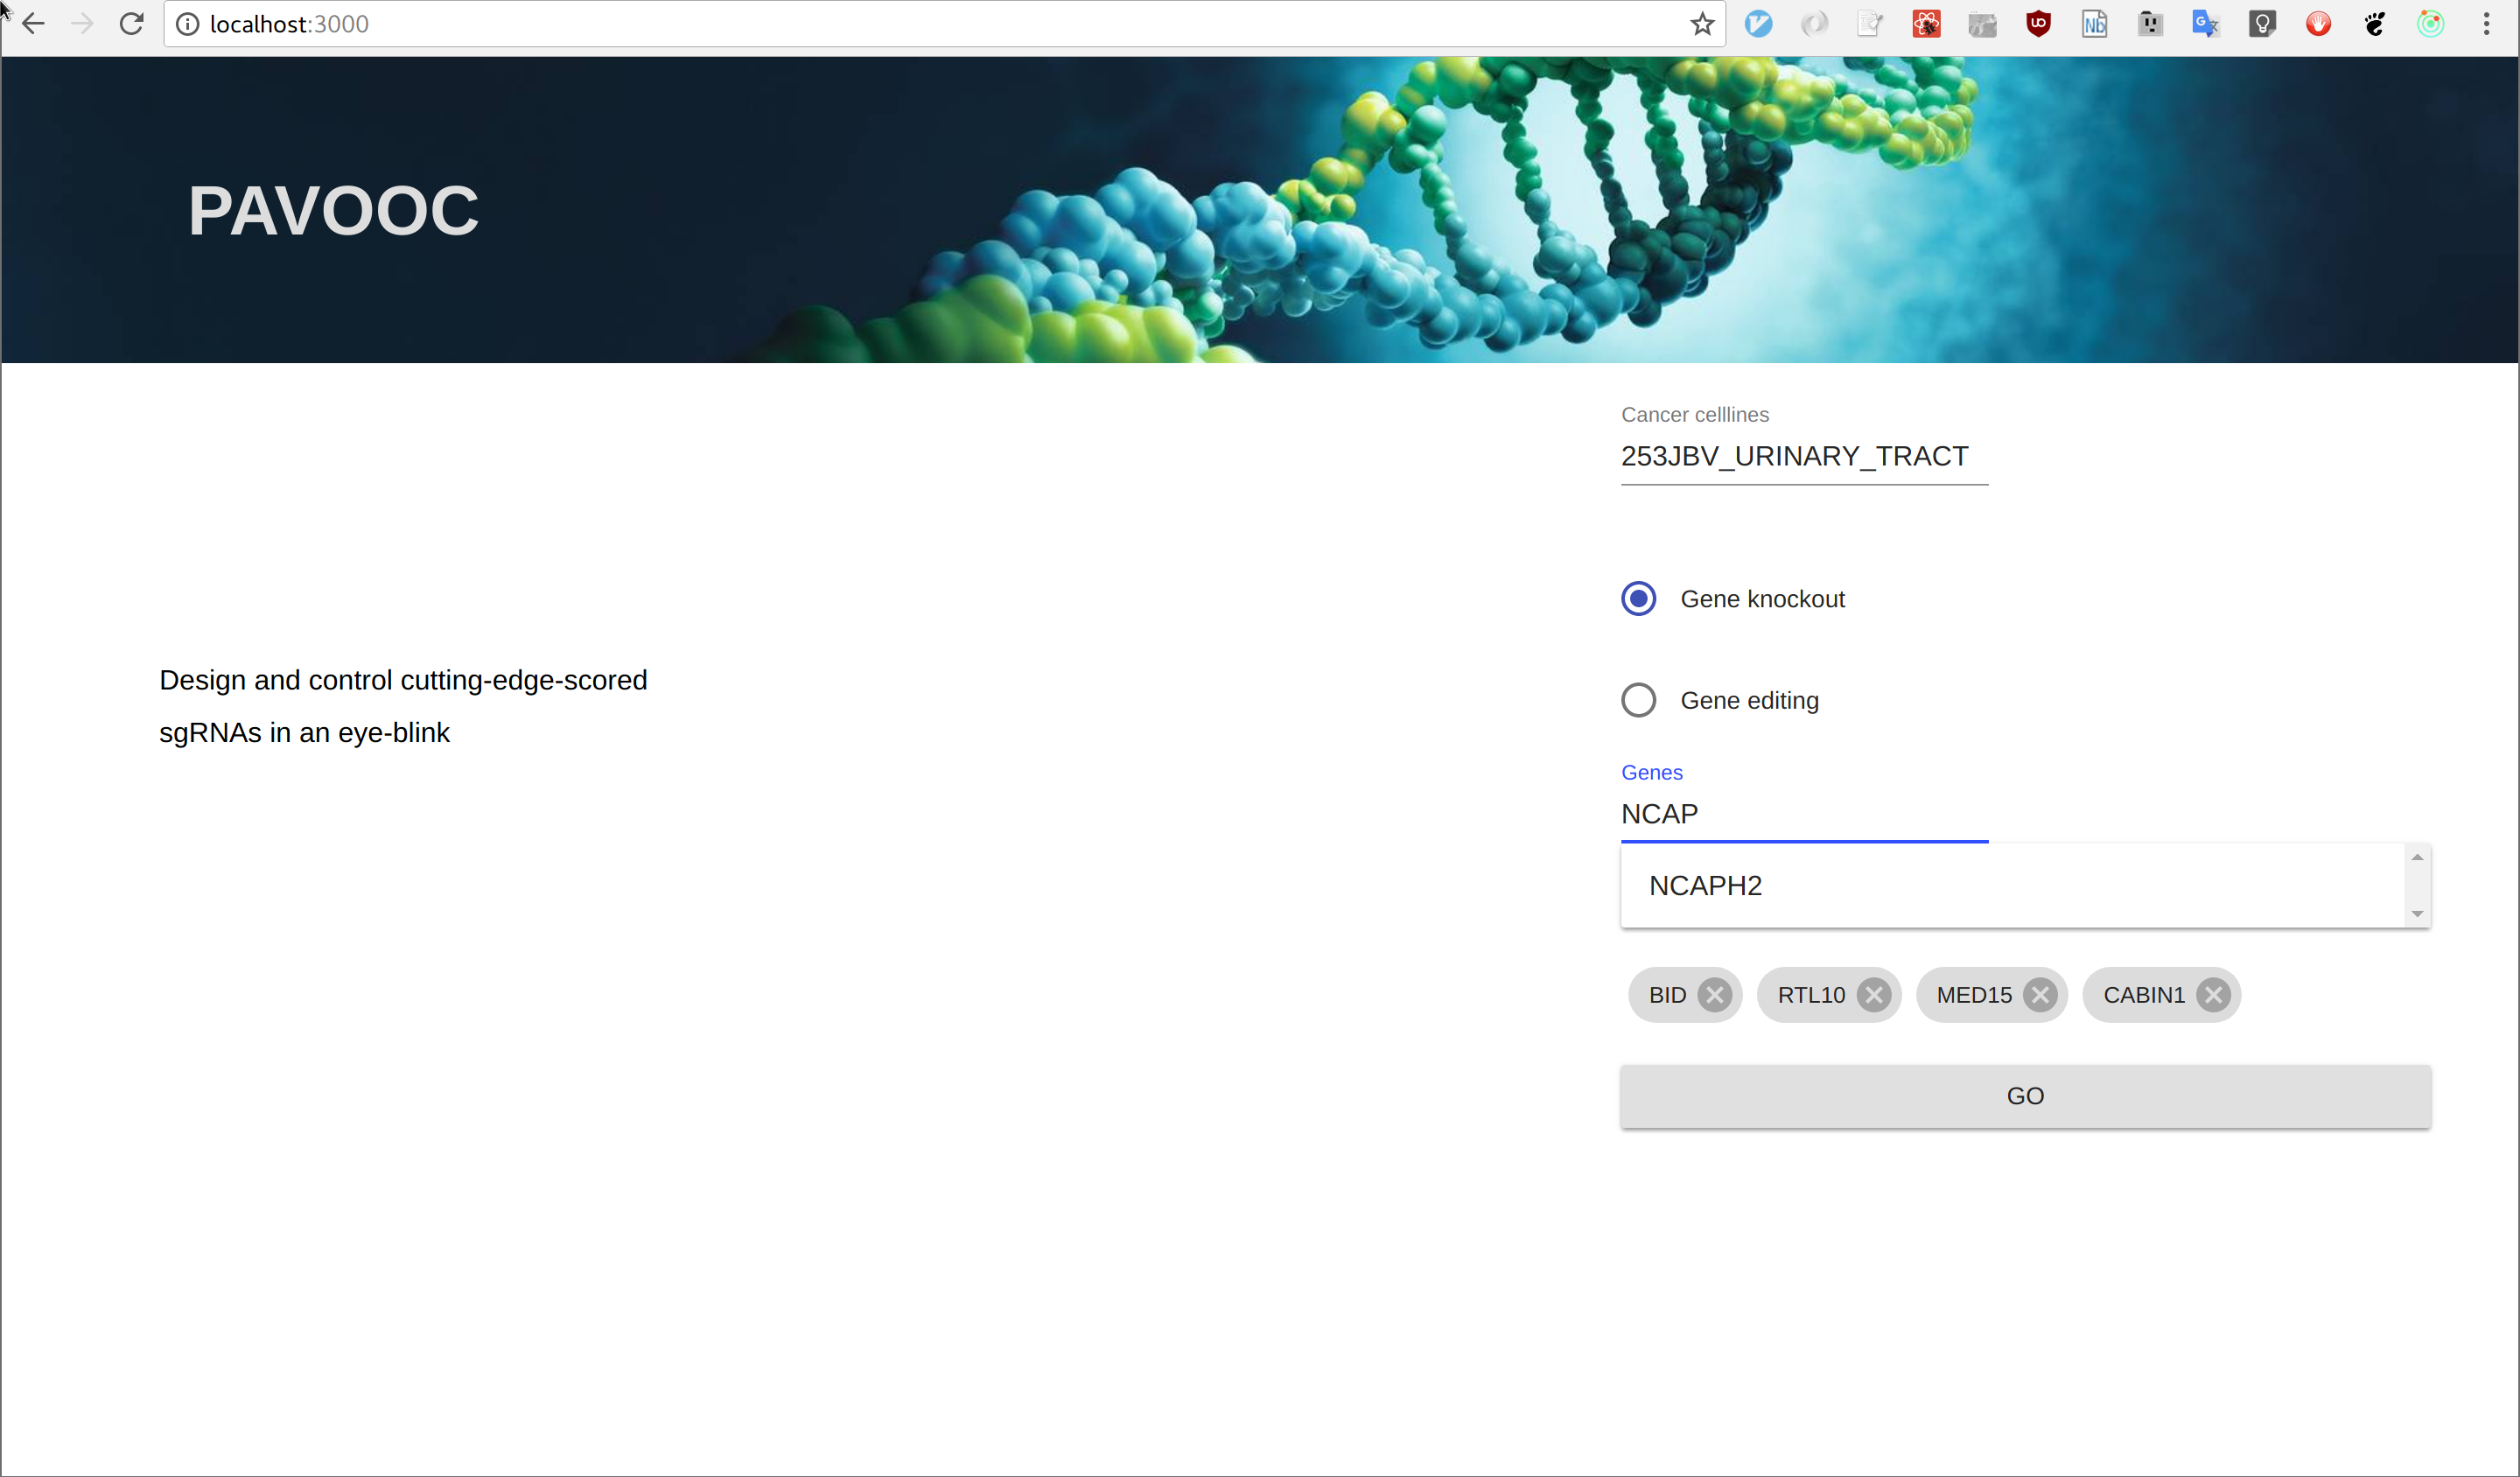
\includegraphics[width=0.8\linewidth]{firstpage.png}
  \end{figure}
\end{frame}

\begin{frame}[fragile]{Application overview}
  \begin{figure}
    \centering
    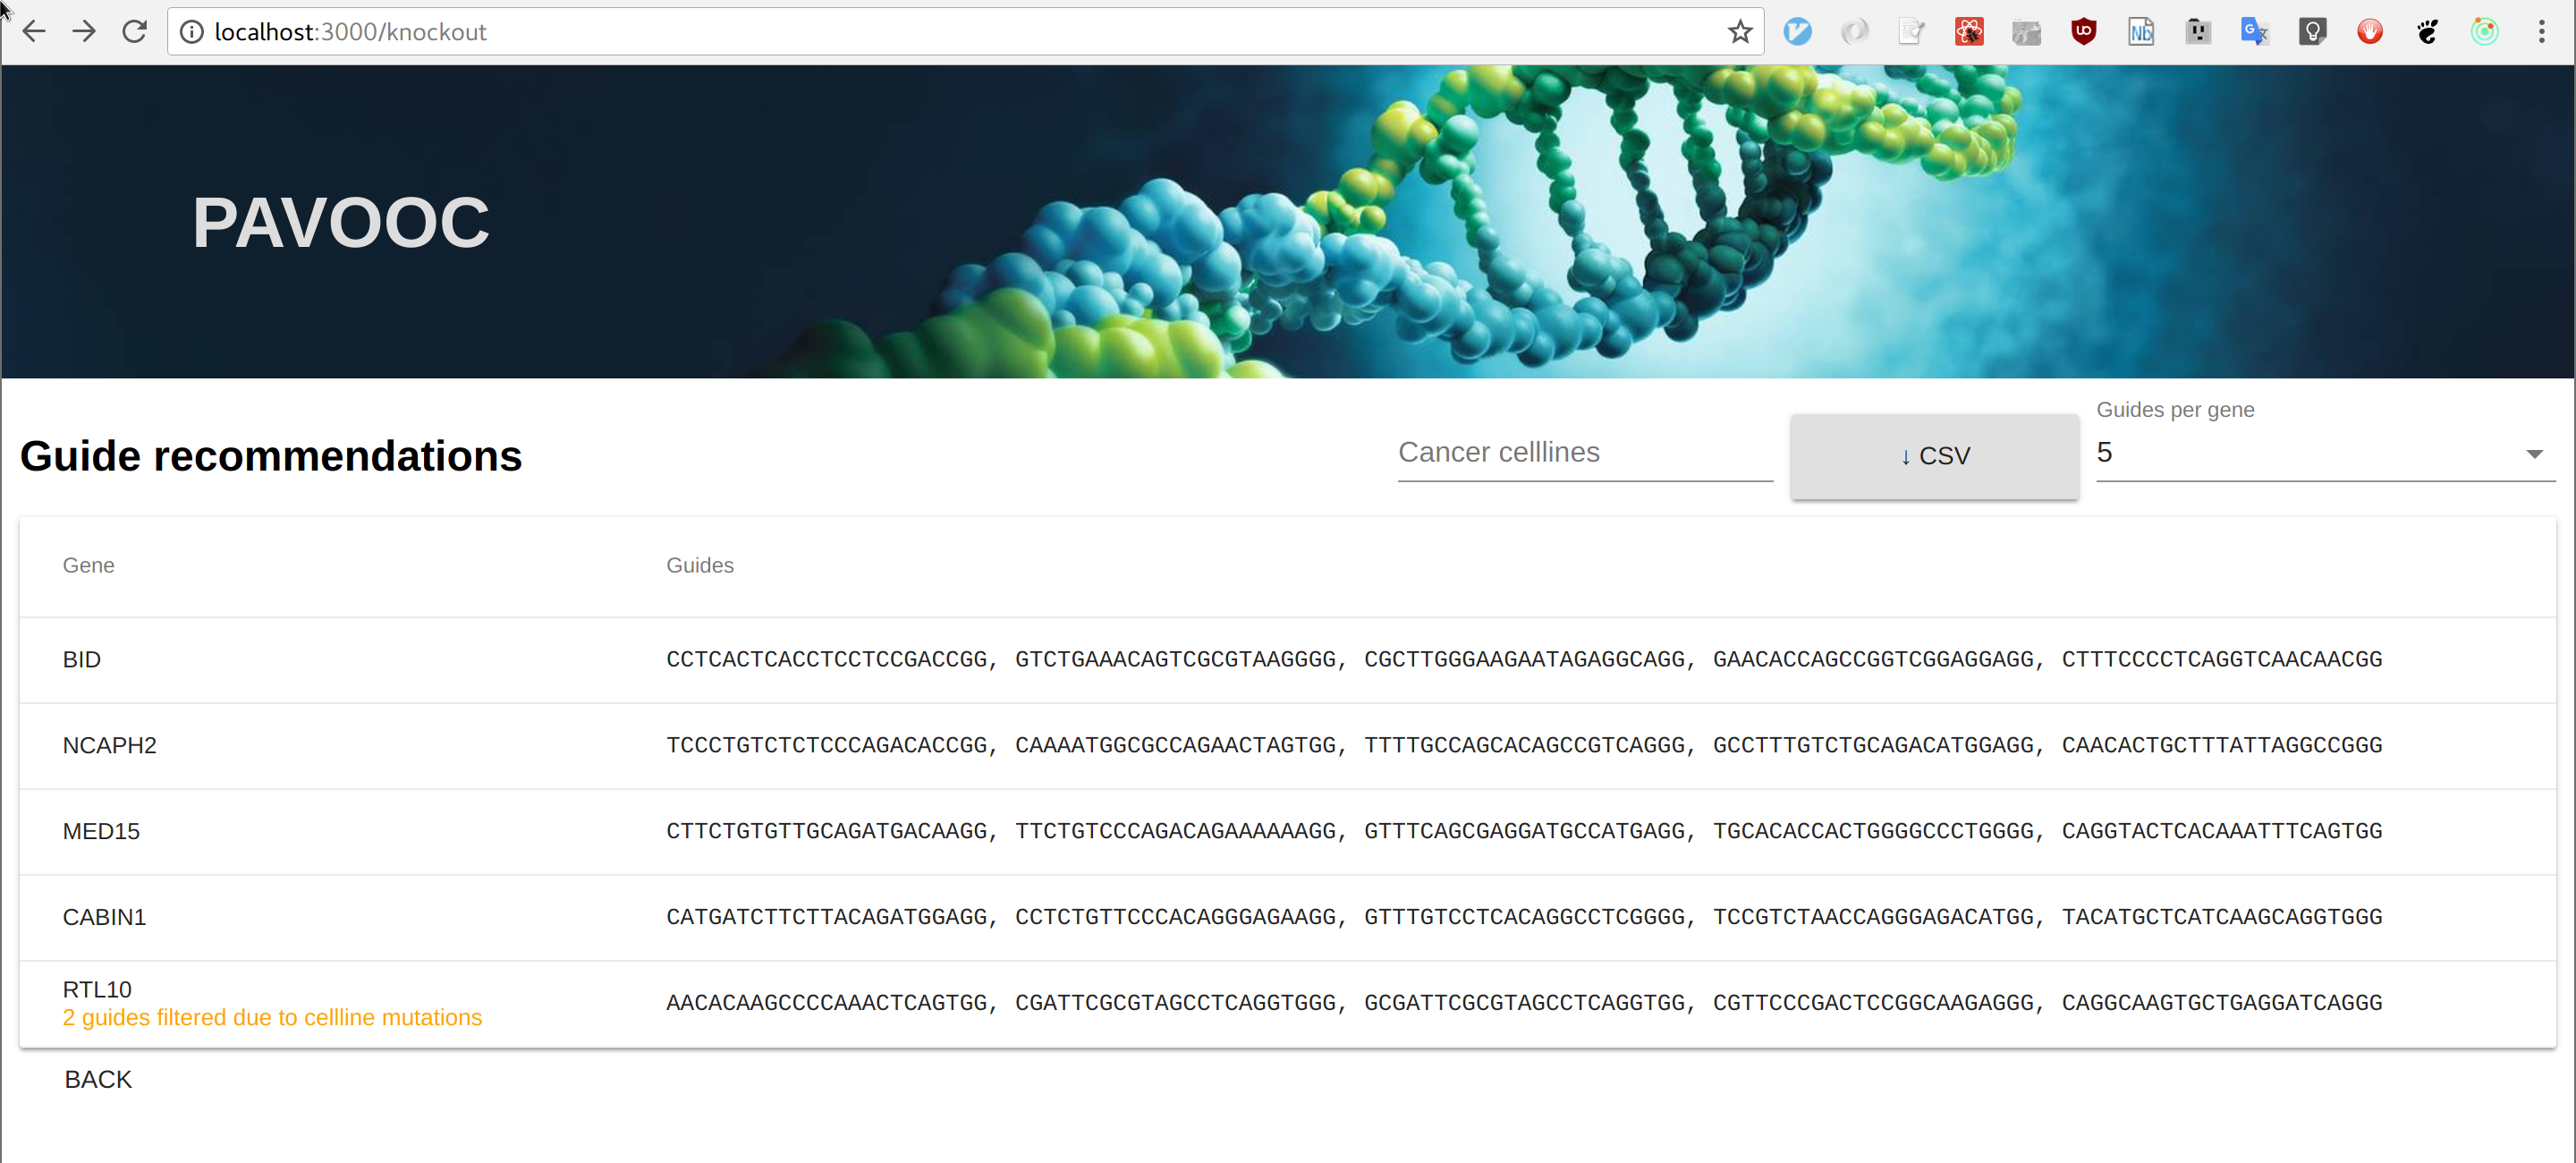
\includegraphics[width=0.8\linewidth]{secondpage.png}
  \end{figure}
\end{frame}


\begin{frame}[fragile]{Application overview}
  \begin{figure}
    \centering
    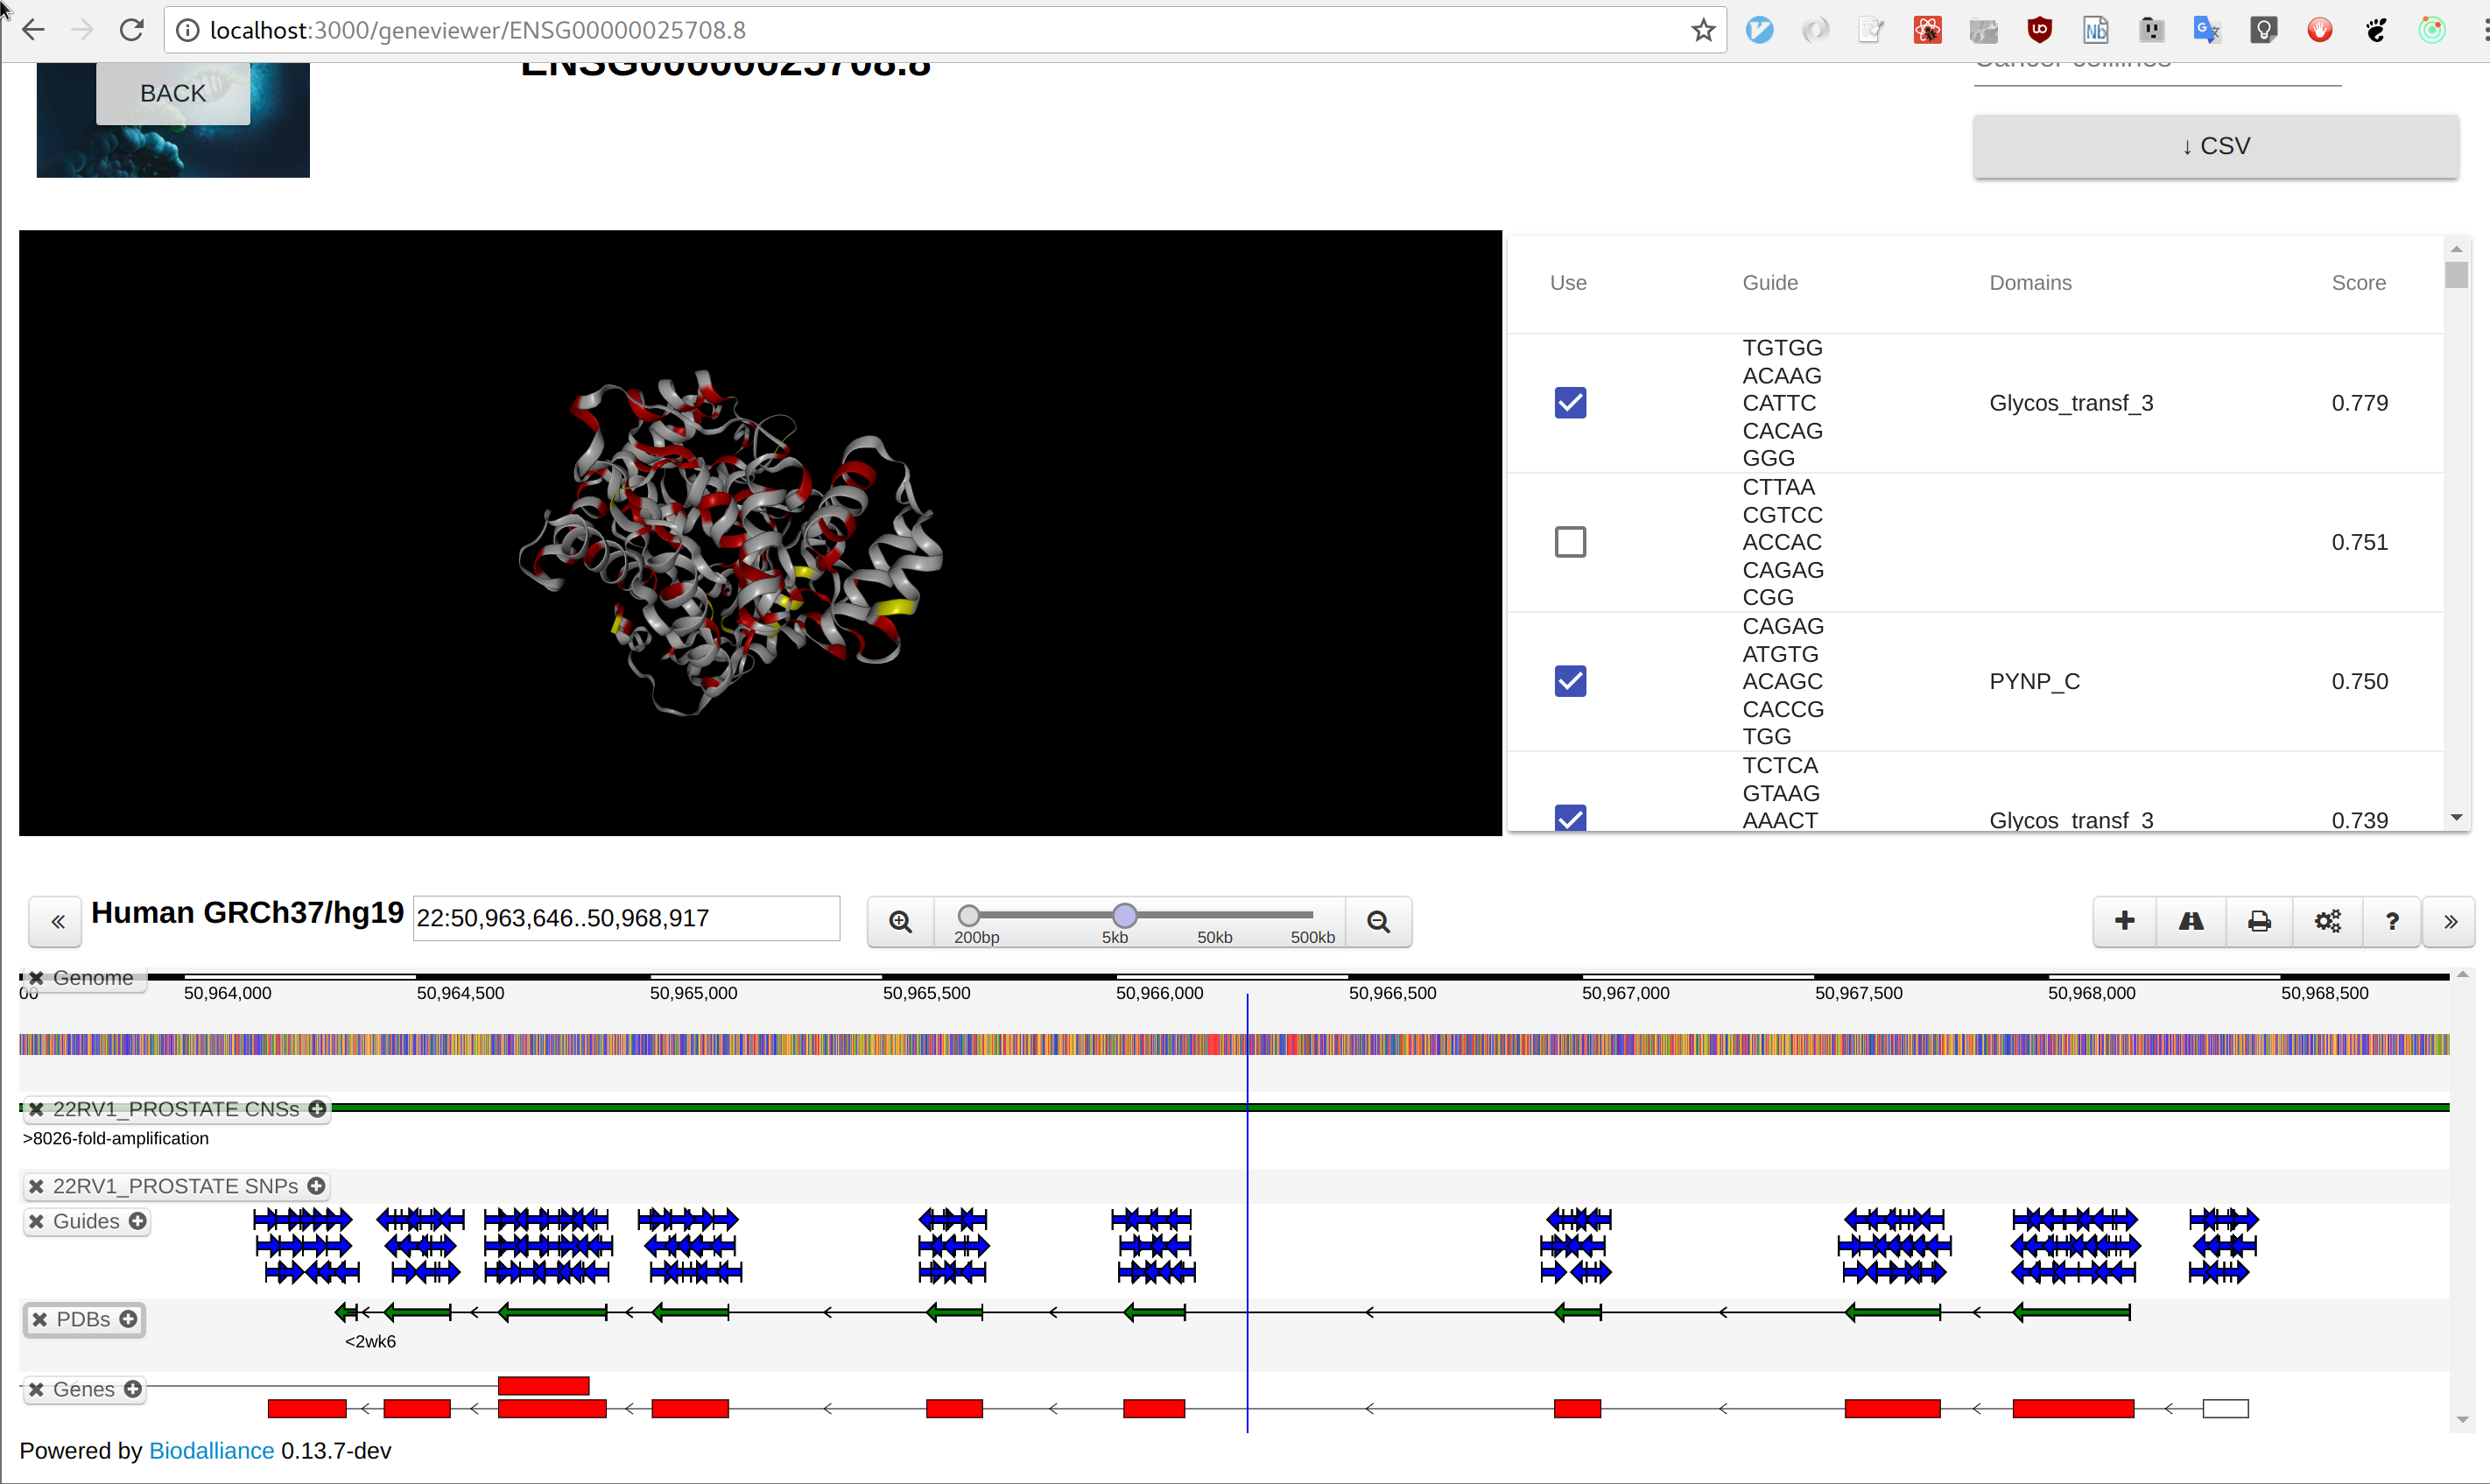
\includegraphics[width=0.8\linewidth]{pagethree.png}
  \end{figure}
\end{frame}

\begin{frame}[fragile]{Application overview}
  \begin{figure}
    \centering
    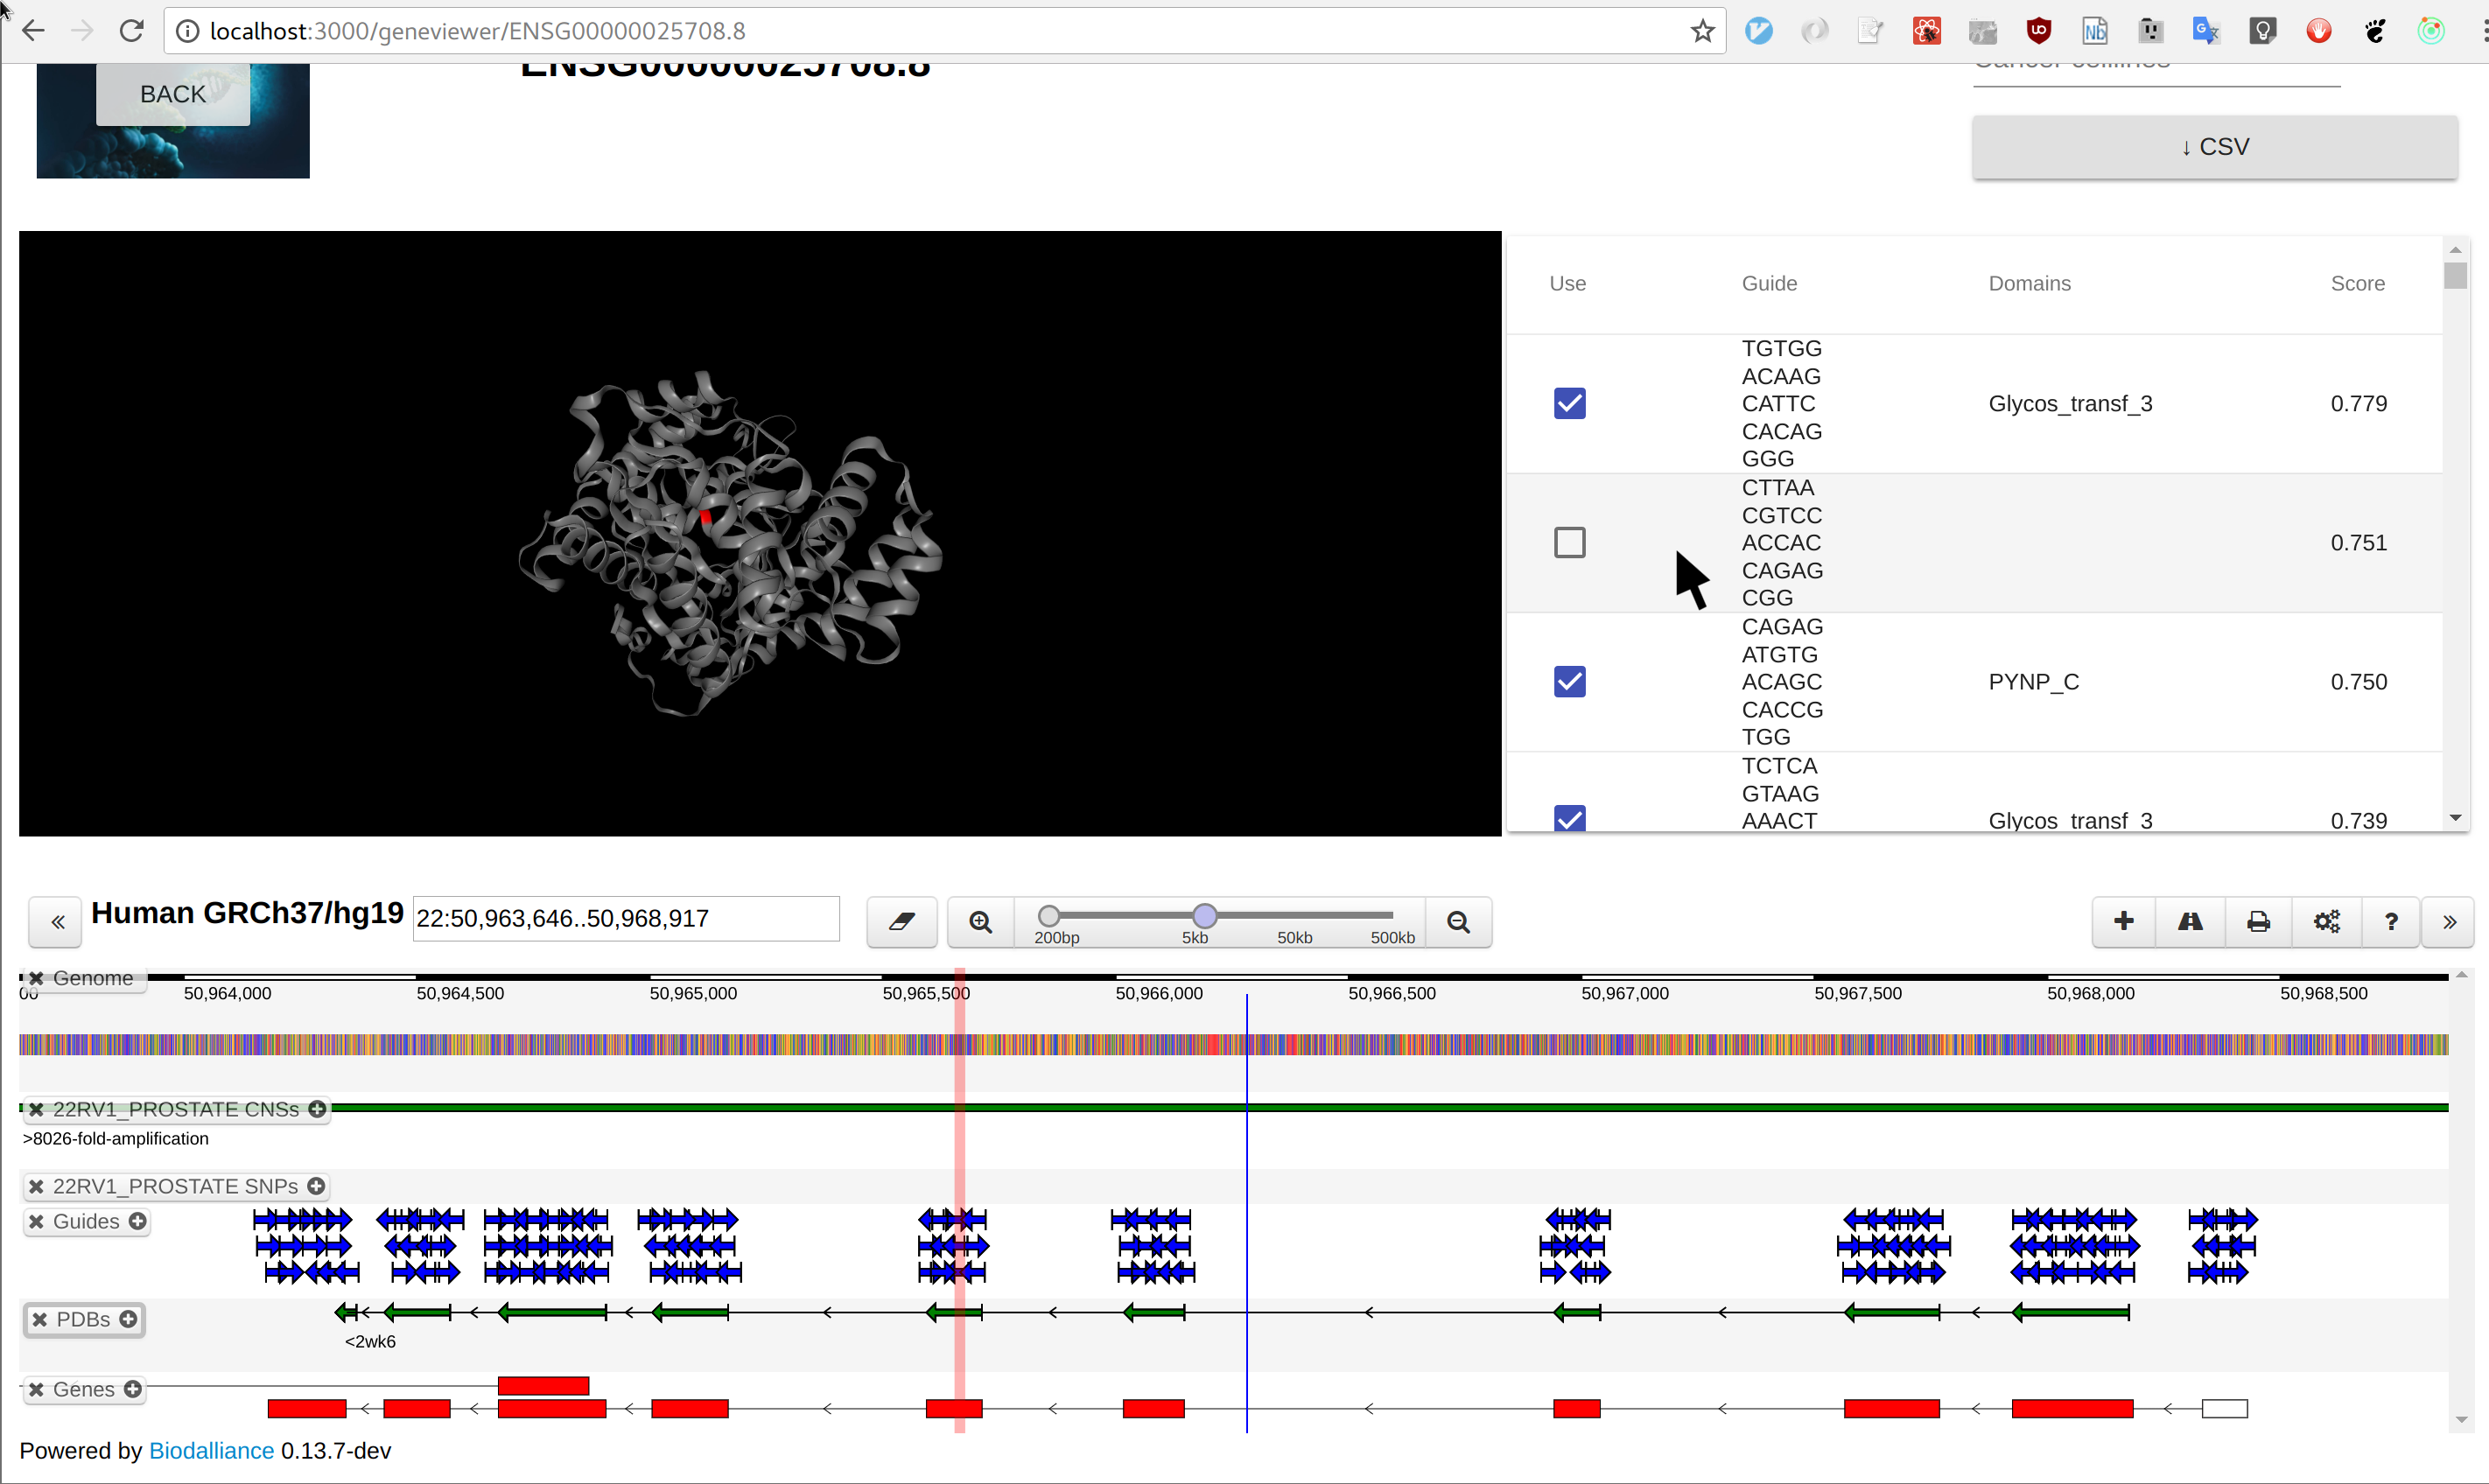
\includegraphics[width=0.8\linewidth]{screen4.png}
  \end{figure}
\end{frame}

\begin{frame}{Acknowledgements}
  \begin{itemize}
    \item Dr.\ Andreas Steffen (supervisor at Bayer)
    \item Prof.\ Manfred Opper (supervisor at TU Berlin)
    \item Dr.\ Djork-Arne Clevert (machine learning scientist at Bayer)
    \item Robin Winter (PhD student at Bayer)
    \item Bayer Pharma AG
  \end{itemize}

\end{frame}
\end{document}
